\subsection{Automatic Subtitles Positioning in 360-Video}

In \cite{mendes2020authoring}, we proposed a model for authoring interactive 360° video. In such a model, we can define interactive 360° video that are presented together with additional information attached to it, such as image, text and spatial audio. The positioning of such additional information is defined by their polar coordinates, start time and duration. Moreover, we can also configure behaviours depending on where the user is looking. For instance, we can define that a text moves with the user's head motion and is always visible or that such text is placed at fixed position if it is in the field of view of the user. Besides the design of such a model, we developed a player that follows the definitions of our model and is able to play interactive 360° video defined by it. Then, we can use \emph{video face clustering} to define the positioning of subtitles according to the actors positioning using our player.

Nowadays, the most common way for representing and transmitting 360-video is using an equirectangular projection~\cite{yang2018object}. With the equirectangular projection, each sphere point is defined by two angles~\cite{snyder1987map}: \emph{latitude}~$\theta \in [-90^{\circ}, +90^{\circ}]$ and \emph{longitude}~$\phi \in [-180^{\circ}, +180^{\circ}]$. This kind of projection creates challenges for image processing and computer vision algorithms, especially to the convolution-based ones because of the severe distortions in areas vertically distant from the center of the image~(see Figure \ref{fig:equirectangular_proj}). Due to these distortions, we adapted the steps of our methods that use traditional CNNs: \emph{Face Detection} and \emph{Embeddings Generation}.

\begin{figure}[!ht]
\centering
    \begin{subfigure}{0.47\linewidth}
        \centering
        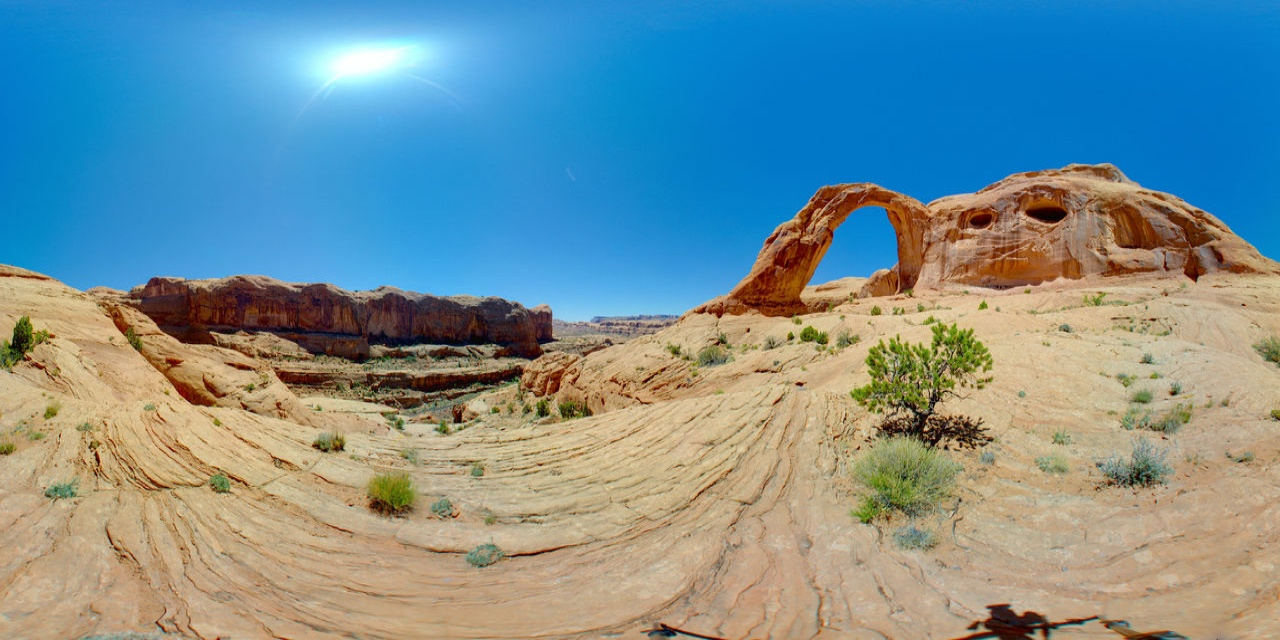
\includegraphics[width=1\textwidth]{img/image (9).jpg}
        \caption{Outdoor equirectangular image.}
        \label{subfig:out_equi}
    \end{subfigure}\hfill
    \begin{subfigure}{0.47\linewidth}
        \centering
        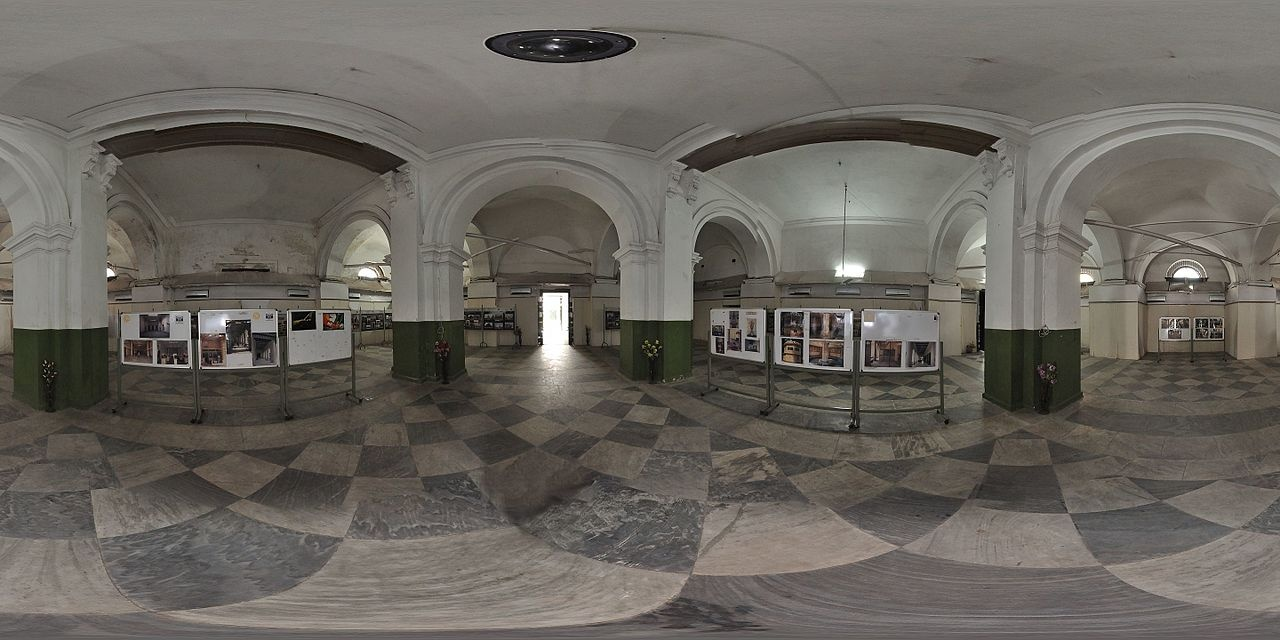
\includegraphics[width=1\textwidth]{img/image (10).JPG}
        \caption{Indoor equirectangular image.}
        \label{subfig:in_equi}
    \end{subfigure}

\caption{Examples of 360-images represented through equirectangular projection.}
\label{fig:equirectangular_proj}
\end{figure}




Because of the distortions present on the equirectangular projection, we opted for elaborating a solution based on viewports extraction. A viewport is defined by its center, in polar coordinates~(lat, long), and its field of view~(FoV). Figure \ref{fig:viewports} shows viewports extracted at different polar coordinates from Figure \ref{subfig:out_equi}.
%%
\begin{figure}[!ht]
    \centering
    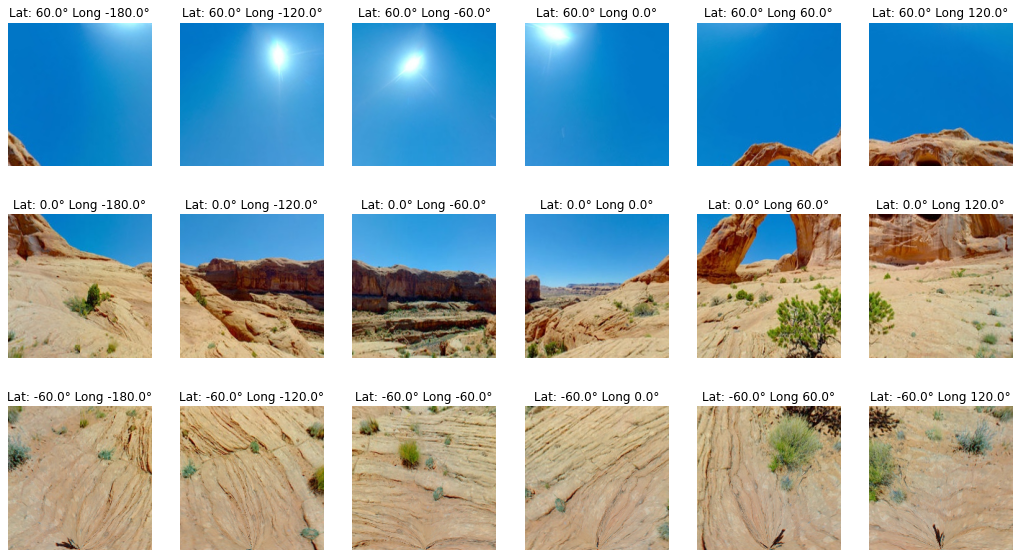
\includegraphics[width=1\textwidth]{img/viewports.png}
    \caption{Viewports extracted at different polar coordinates with $FoV = 60^{\circ}$}
    \label{fig:viewports}
\end{figure}
%%
For each viewport, we apply a face detection model. 
Then, we project the faces detected bounding boxes back to the equirectangular image. 
%%
After eliminating repeated detections with NMS, we perform \emph{Embeddings Generation} using the faces detected in the viewports~(with reduced distortions) instead of using its equivalent in the original equirectangular video frame.

By using these adaptations to the 360-video domain, we are able to apply \emph{video face clustering} to them and obtain the spatiotemporal localization of actors. With this in hands, we can automatically position subtitles close to the actors in the 360-video using our authoring model (see Figure \ref{subfig:subtitles_actor}). Moreover, as our authoring model supports interactivity, we can detect whether actors are in the FOV of the user. We can use this information to place subtitles in the bottom of the user's FOV when the actor speaking is not visible to the user. Thus, the subtitles are always visible to the user.


\begin{figure}[!ht]
\centering
    \begin{subfigure}{0.47\linewidth}
        \centering
        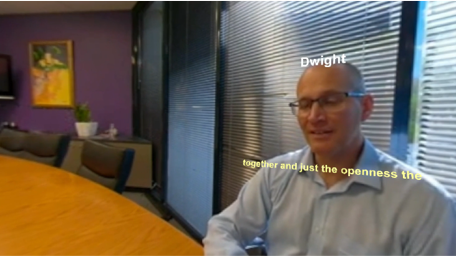
\includegraphics[width=1\textwidth]{img/video360/subtitles_actor.png}
        \caption{Subtitles positioning close to actors' face when they are in the user's FOV.}
        \label{subfig:subtitles_actor}
    \end{subfigure}\hfill
    \begin{subfigure}{0.47\linewidth}
        \centering
        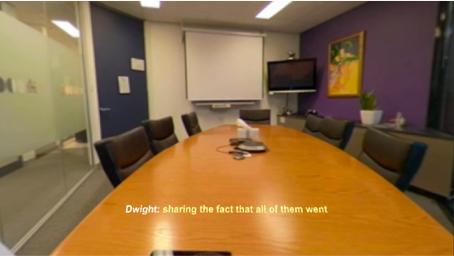
\includegraphics[width=1\textwidth]{img/video360/subtitles_bottom.png}
        \caption{Subtitles positioning in the bottom of user's FOV.}
        \label{subfig:subtitles_bottom}
    \end{subfigure}

\caption{Subtitles positioning using video face clustering and our authoring model.}
\label{fig:subtitles}
\end{figure}

Regarding this application, we point out the following remaining task:

\begin{itemize}
    \item T1 - Organize and tabulate evaluation results of face detection in equirectangular images.
\end{itemize}